\section{Preliminaries}
We introduce the definitions of the Clarke subdifferential and various approximate Clarke stationarity points for general locally Lipschitz functions.

Let $F:\RR^d\to\RR$ be locally Lipschitz. The Clarke subdifferential of
$F$ at $\bx$ is denoted by $\partial_C F(\bx)$~\citep{clarke1990optimization}.
A point $\bx$ is called an $\varepsilon$-Clarke stationary point if
\[
    \operatorname{dist}\bigl(\zero,\partial_C F(\bx)\bigr)
    \leq \varepsilon .
\]
For general nonsmooth nonconvex functions, such a same-point certificate
is not a finite-time target in the worst case. This motivates the
Goldstein-type relaxation below~\citep{goldstein1977optimization,Zhang-2020-Complexity}.

\begin{figure}[t]
    \centering
    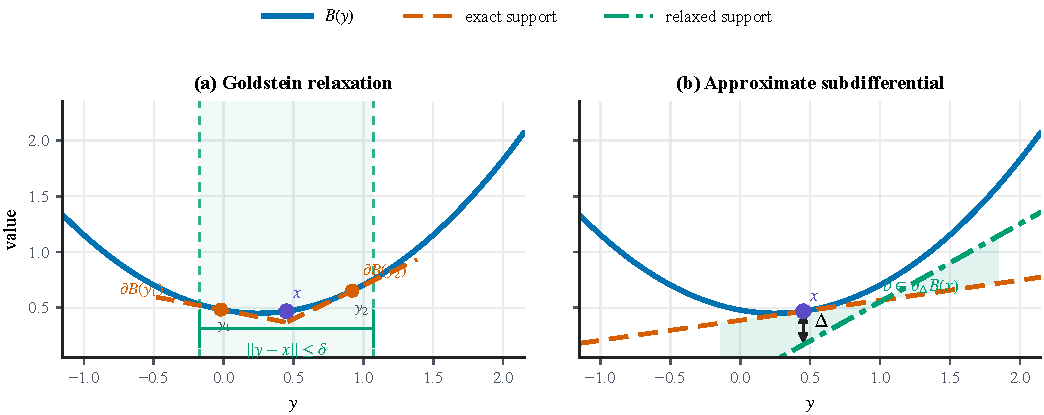
\includegraphics[width=\textwidth]{goldstein_vs_approximate_subdifferential.pdf}
   \caption{The Goldstein subdifferential $\partial^G_\delta$ and the
$\delta$-subdifferential $\partial_\delta$ relax exact stationarity along different axes. The former convexifies exact subgradients collected over the ball $\mathcal{B}_\delta(\bar{\bx})$ (a spatial enlargement), while the
latter fixes the base point and tolerates a Fenchel--Young gap of at most
$\delta$ in the supporting inequality (a value relaxation).}
    \label{fig:goldstein-vs-approximate-subdifferential}
\end{figure}

